\documentclass[11pt,a4paper]{article}
\usepackage[T1]{fontenc}
\usepackage[utf8]{inputenc}
\usepackage{lmodern}
\usepackage{amsmath,amssymb,amsthm,mathtools,mathrsfs}
\usepackage{graphicx,float,xcolor,multicol}
\usepackage[shortlabels]{enumitem}
\usepackage[margin=27mm]{geometry}
\usepackage{microtype,needspace,placeins}
\usepackage{tikz,tikz-cd}
\usetikzlibrary{arrows.meta,calc,positioning,patterns,decorations.pathreplacing}
\usepackage[colorlinks=true,linkcolor=teal,urlcolor=teal,citecolor=teal]{hyperref}
\setlength{\parindent}{0pt}
\setlength{\parskip}{.6em}
\setcounter{secnumdepth}{0}
\allowdisplaybreaks
\raggedbottom
\providecommand{\cross}{\times}
\DeclareUnicodeCharacter{2020}{\ensuremath{\dagger}}
\DeclareMathOperator{\supp}{supp}
\DeclareMathOperator*{\esssup}{ess\,sup}
\providecommand{\chapter}{\section}
\newenvironment{tool}[2]{\subsection*{Tool #1 --- #2}}{}
\newcommand{\ToolRef}[1]{Tool #1}
\newcommand{\FigureTag}[2]{\textit{Figure #1}}
\newcommand{\Result}[1]{\subsection*{#1}}
\newcommand{\Application}[1]{\subsubsection*{Application\if\relax\detokenize{#1}\relax\else\space--- #1\fi}}
\newcommand{\ProofHeading}{\par\textit{Proof.}\space}
\newcommand{\ProofOf}[1]{\par\textit{Proof of #1.}\space}
\newcommand{\RemarkHeading}{\par\textbf{Remark.}\space}
\newcommand{\NoteHeading}{\par\textbf{Note.}\space}
\newcommand{\ExerciseHeading}{\par\textbf{Exercise.}\space}

\graphicspath{{figures/complex-analysis/}}
\begin{document}
\section*{Keyhole Contour Construction}
% BLOG-CONTENT-BEGIN
Now let us resume our exposition on complex analysis (singularities), which we left in the middle to develop the notions of interior and exterior. We did that first because, to talk about a point where the function is ``yet not defined'' or ``can never be defined,'' we need some curve $\gamma$ with the point $z_0\in\operatorname{int}(\gamma)$. Thus, exploiting the regularity of $f$ (which, as we saw before, is merely the fact that the boundary values of $f$ fix the values in the interior), one may, if possible, extend the analyticity of $f$ to $z_0$. We shall mostly deal with isolated singularities; in other words, punctures in the domain. The basic philosophy that helps settle the matter of isolated singularities is:

\begin{quote}
If $f$ can be extended and the gaps in its domain can be filled, then it can and must be done with the help of the boundary of a set containing those punctures in its interior, because certainly the extended function is regular.
\end{quote}

Digest this!

Let us return to our applied function
\[
  \frac{f(z)}{z-z_0},
  \qquad f\in H(U),\quad z_0\in\mathbb C.
\]
We saw before that
\[
  \int_\gamma \frac{f(z)}{z-z_0}\,dz
  =f(z_0)\int_\gamma\frac{dz}{z-z_0}
  \qquad (\forall z_0\in U\setminus\gamma^*),
\]
and we also saw that
\[
  g(z_0):=\int_\gamma\frac{f(z)}{z-z_0}\,dz
\]
is a holomorphic function of $z_0$; in fact, $g\in H(\mathbb C\setminus\gamma^*)$. One must just find a way to see that
\[
  \left.g\right|_{U\setminus\gamma^*}=f.
\]


Then one can extend $f$ to fill in the punctures via \emph{keyhole contour integration}. There are several crucial constructions in complex analysis; of them all, the construction of a keyhole contour is foundational. Let us do that first. The idea of the extension shall become clear as we proceed with this exposition.

\subsection*{Tool 25 — Keyhole Contour Construction}

Given two polygonal paths $\gamma_1$ and $\gamma_2$ such that \(\gamma_2\subset \operatorname{int}(\gamma_1),\)
there exists a simple closed polygonal path $\gamma_\varepsilon$ such that
\[
  \lim_{\varepsilon\to0}\gamma_\varepsilon
  \equiv_{\mathrm{UR}}\gamma_1+(-\gamma_2).
\]
Here UR denotes equality up to reparametrization, and $\gamma_1$ and $\gamma_2$ are oriented anticlockwise.


These $\gamma_\varepsilon$ are the ``keyholes'' which, under a pointwise limit, collapse to $\gamma_1+(-\gamma_2)$.

\begin{figure}[htbp]
  \centering
  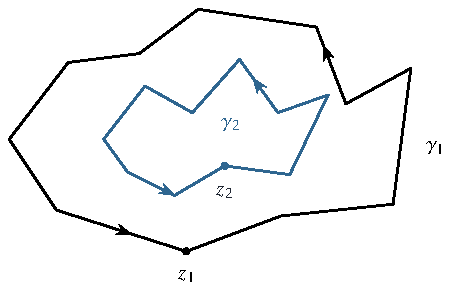
\includegraphics[width=.51\textwidth]{note7-fig-01.pdf}
  \textit{Figure N7.1}
\end{figure}

\textit{Proof.}
The set \(\operatorname{ext}(\gamma_2)\cap\operatorname{int}(\gamma_1)\)
is a domain. We also note that
\[
  \partial\bigl(\operatorname{ext}(\gamma_2)\cap\operatorname{int}(\gamma_1)\bigr)
  =\gamma_1^*\cup\gamma_2^*.
\]
Thus
\[
  \gamma_1^*\cup
  \bigl(\operatorname{ext}(\gamma_2)\cap\operatorname{int}(\gamma_1)\bigr)
  \cup\gamma_2^*
\]
is connected. Pick two points $z_1\in\gamma_1^*$ and $z_2\in\gamma_2^*$. Let \(d=\operatorname{dist}(\gamma_1,\gamma_2).\)
Choose $\varepsilon_1,\varepsilon_2<d$, and choose
\[
  w_1\in B_{\varepsilon_1}(z_1),
  \qquad
  w_2\in B_{\varepsilon_2}(z_2),
\]
such that $w_i\in\operatorname{ext}(\gamma_2)\cap\operatorname{int}(\gamma_1)$. There is a path between $w_1$ and $w_2$; approximate it by a polygonal path $\gamma_{w_1,w_2}$ in $\operatorname{ext}(\gamma_2)\cap\operatorname{int}(\gamma_1)$. Notice that
\[
  \gamma_{z_2\to w_2}^*\setminus\{z_2\}
  \subset \operatorname{ext}(\gamma_2)\cap\operatorname{int}(\gamma_1),
\]
and similarly
\[
  \gamma_{w_1\to z_1}^*\setminus\{z_1\}
  \subset \operatorname{ext}(\gamma_2)\cap\operatorname{int}(\gamma_1).
\]
Let
\[
  \Omega=\operatorname{ext}(\gamma_2)\cap\operatorname{int}(\gamma_1),
\]
and consider a tube around the polygonal path
\[
  \gamma_{z_2\to w_2}+\gamma_{w_1,w_2}+\gamma_{w_1\to z_1}=:\gamma_p.
\]
Following the complex tube lemma, one can arrange matters so that the tube has polygonal boundary with sides parallel to $\gamma_p$.


Transform $\mathbb C$ so that the edge on which $z_1$ lies becomes the $x$-axis, with one of its vertices at the origin. Now shift $\gamma_p$ by $\varepsilon$ so that $\gamma_p+\varepsilon$ belongs to the tube, and let it intersect $\gamma_1$ and $\gamma_2$ at $y_1$ and $y_2$. Orient appropriately to obtain a keyhole.

\begin{figure}[H]
  \centering
  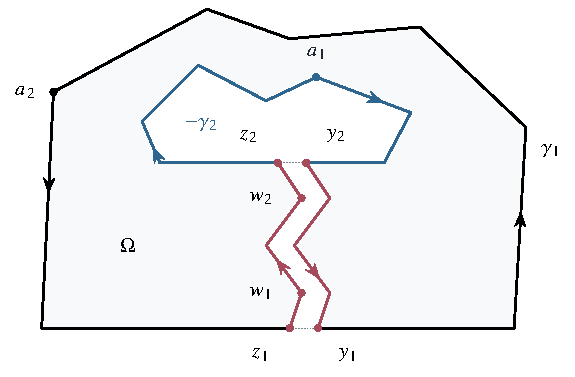
\includegraphics[width=.70\textwidth]{note7-fig-02.pdf}
  \textit{Figure N7.2}
\end{figure}

The keyhole is
\[
  \gamma_\varepsilon
  :=\gamma_{z_2\to a_1}
  +\left.\gamma_1\right|_{a_1\to y_2}
  +\gamma_{y_2\to y_1}
  +\gamma_{y_1\to a_2}
  +\gamma_{a_2\to z_1}
  +\gamma_{z_1\to z_2}.
\]


\textbf{Exercise.} Similarly construct a multiple keyhole.

\textbf{Remark.} The reason it is called a keyhole, even though it might look like neither a keyhole nor even a hole to begin with, is that it rather looks like, or has a similar orientation switch as, a keyhole.

\begin{figure}[H]
  \centering
  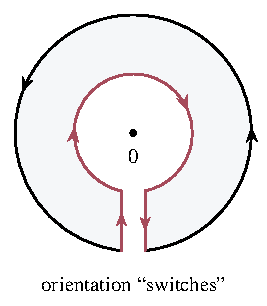
\includegraphics[width=.30\textwidth]{note7-fig-03.pdf}
  \textit{Figure N7.3}
\end{figure}


Now let us say that we have a domain like this, with a big puncture. Let $\gamma_1$ and $\gamma_2$ be polygonal paths winding around the puncture, with
\[
  \gamma_2\subset\operatorname{int}(\gamma_1).
\]
In particular,
\[
  \operatorname{ext}(\gamma_2)\cap\operatorname{int}(\gamma_1)\subset U.
\]

\begin{figure}[H]
  \centering
  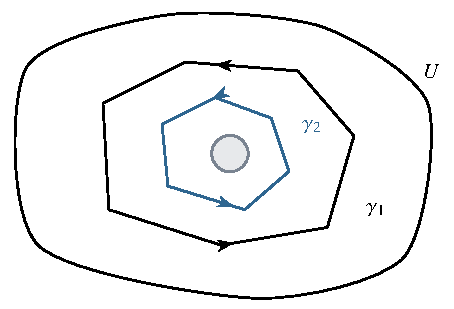
\includegraphics[width=.48\textwidth]{note7-fig-04.pdf}
  \textit{Figure N7.4}
\end{figure}

Let $z\in\operatorname{int}(\gamma_1)\cap\operatorname{ext}(\gamma_2)$. Then
\[
  W_{\gamma_1}(z)=1,
  \qquad
  W_{\gamma_2}(z)=0.
\]
Also, by taking keyholes one can argue that
\[
  \int_{\gamma_1}f(z)\,dz=\int_{\gamma_2}f(z)\,dz,
  \qquad f\in H(U).
\]
In particular, the same is true for the spiked function
\[
  \frac{f(z)-f(z_0)}{z-z_0},
  \qquad z_0\in\operatorname{int}(\gamma_1)\cap\operatorname{ext}(\gamma_2).
\]
We thus have
\begin{align*}
  \frac{1}{2\pi i}\int_{\gamma_1}\frac{f(w)-f(z_0)}{w-z_0}\,dw
  &=\frac{1}{2\pi i}\int_{\gamma_2}\frac{f(w)-f(z_0)}{w-z_0}\,dw,\\
  f(z_0)
  &=\frac{1}{2\pi i}\int_{\gamma_1}\frac{f(w)}{w-z_0}\,dw
    -\frac{1}{2\pi i}\int_{\gamma_2}\frac{f(w)}{w-z_0}\,dw.
\end{align*}
We noticed above that
\[
  \frac{1}{2\pi i}\int_{\gamma_1}\frac{f(w)}{w-z_0}\,dw
\]
is holomorphic on $\mathbb C\setminus\gamma_1^*$. This barrier of the curve is what we eradicated by putting another curve inside $\gamma_1$.

Now put
\[
f_1(z):=
\begin{cases}
\displaystyle \frac{1}{2\pi i}\int_{\gamma_1}\frac{f(w)}{w-z}\,dw,
  &z\in\operatorname{int}(\gamma_1),\\[1.2ex]
\displaystyle f(z)+\frac{1}{2\pi i}\int_{\gamma_2}\frac{f(w)}{w-z}\,dw,
  &z\in U\cap\operatorname{ext}(\gamma_2),
\end{cases}
\]
and
\[
f_2(z):=
\begin{cases}
\displaystyle -\frac{1}{2\pi i}\int_{\gamma_2}\frac{f(w)}{w-z}\,dw,
  &z\in\operatorname{ext}(\gamma_2),\\[1.2ex]
\displaystyle f(z)-\frac{1}{2\pi i}\int_{\gamma_1}\frac{f(w)}{w-z}\,dw,
  &z\in U\cap\operatorname{int}(\gamma_1).
\end{cases}
\]
Then
\[
  f_1\in H(\operatorname{int}(\gamma_1)),
  \qquad
  f_2\in H(\operatorname{ext}(\gamma_2)),
\]
and on $\operatorname{int}(\gamma_1)\cap\operatorname{ext}(\gamma_2)$, \(f(z)=f_1(z)+f_2(z).\)
Note that $f_1$ and $f_2$ are defined on two separate domains and are patched together by $f(z)$.


\textbf{Remark.} Although $f_1\in H(\mathbb C\setminus\gamma_1^*)$, we did not use the full power of the continuation of the integral, because we needed it to connect to $f(z)$. So we used $\operatorname{int}(\gamma_1)\cap\operatorname{ext}(\gamma_2)$ as the gluing domain where $f$ is existing, defined, and analytic. Notice that there is no gluing domain with which to extend $f_1$ beyond $\operatorname{int}(\gamma_1)$, because the decomposition is true only in the domain $\operatorname{int}(\gamma_1)\cap\operatorname{ext}(\gamma_2)$. Or, we have to consider another $\gamma_0$ in $U$ such that $\gamma_1\subset\operatorname{int}(\gamma_0)$, which is in some sense what we already have with $\gamma_1$ and $\gamma_2$.

\textbf{Remark.} Note that $|f_2(z)|\to0$ as $|z|\to\infty$, since $\gamma_2$ is compact. Thus the decomposition is unique. Suppose not: let \(f=f_1+f_2=g_1+g_2,\)
with $f_2,g_2\to0$ as $|z|\to\infty$. Then
\[
  f_1-g_1=g_2-f_2
\]
on a domain in $U$. Hence $g_2-f_2$ is entire and tends to $0$ as $z\to\infty$, so $g_2=f_2+c$ and $f_1=g_1+c$. But as $z\to\infty$, $c\to0$; therefore $c=0$, $g_2=f_2$, and $f_1=g_1$. Hence the decomposition is unique.

\textbf{Remark.} By induction one can extend this result. Let $\gamma_0,\{\gamma_i\}_{i=1}^n$ be Jordan curves such that
\[
  \gamma_i^*\cap\gamma_j^*=\varnothing,
  \qquad
  \gamma_i^*\subset\operatorname{int}(\gamma_0)
  \quad(\forall i,j),
\]
and
\[
  \operatorname{int}(\gamma_i)\cap\operatorname{int}(\gamma_j)=\varnothing
  \quad(i\ne j).
\]
Let
\[
  \Omega=\operatorname{int}(\gamma_0)\cap\bigcap_i\operatorname{ext}(\gamma_i).
\]
Then, if $f\in H(U)$,
\[
  f(z)=\frac{1}{2\pi i}\int_{\gamma_0}\frac{f(w)}{w-z}\,dw
  -\sum_{j=1}^n\frac{1}{2\pi i}\int_{\gamma_j}\frac{f(w)}{w-z}\,dw.
\]


A geometric digression is much needed to explain how this decomposition, or the keyhole contour integration method in general, can fix holes.

\subsection*{Proposition}

Let a simple circular closed path be a concatenation of finitely many circular arcs. Given disks $D_1,D_2,\ldots,D_n$ such that $\bigcup_iD_i$ is connected, prove that
\[
  \partial\Bigl(\bigcup_iD_i\Bigr)
  =\bigsqcup_{j=0}^{k}\gamma_{c_j},
\]
where the $\gamma_{c_j}$ are circular paths such that
\[
  \gamma_{c_j}^*\cap\gamma_{c_\ell}^*=\varnothing,
  \qquad
  \operatorname{int}(\gamma_{c_0})\supset\gamma_{c_j}^*,
\]
and
\[
  \operatorname{int}(\gamma_{c_j})\cap\operatorname{int}(\gamma_{c_\ell})
  =\varnothing
  \qquad (j,\ell\ge1,\ j\ne\ell).
\]
In short, if $\bigcup_iD_i$ is connected, we have the setup needed to decompose any
\[
  f\in H\Bigl(\bigcup_iD_i\Bigr).
\]
\emph{(Draw!)}

\textit{Proof.}
Let us do this via induction. For $n=2$, it is evident. Let it be true for $n=k$. Consider $n=k+1$. Note that $\partial D_{k+1}$ will either belong to $\operatorname{int}(\gamma_{c_j})$ or to $\operatorname{ext}(\gamma_{c_j})$. The curve $\gamma_{c_j}$ will cut $\partial D_{k+1}$ at finitely many points; call them $d_1,d_2,\ldots,d_r$. Look at two consecutive points $d_i$ and $d_{i+1}$, where the $d_i$ are arranged in increasing argument, under a WLOG assumption that $D_{k+1}=S^1$.

Let $\gamma_{c_0}$ cut $\partial D_{k+1}$ at $d_i$ and $d_j$. Then the minor and major arcs will belong, respectively, to the interior and exterior (or the other way around) of $\gamma_{c_0}$. Consider the arc that belongs to the exterior, and replace the portion of $\gamma_{c_0}$ in $D_{k+1}$ by that arc. None of the arcs $\gamma_{c_j}$, $j>1$, will intersect that arc, since
\[
  \gamma_{c_j}^*\cap\operatorname{ext}(\text{new }\gamma_{c_0})=\varnothing,
\]
and hence
\[
  \operatorname{int}(\gamma_{c_0})
  \subset\operatorname{int}(\text{new }\gamma_{c_0}).
\]
By a connectedness argument, note that if $\gamma_{c_j}$, $j>1$, cuts $\partial D_{k+1}$ at $d_i$ and $d_\ell$, then $|i-\ell|=1$.


Now one can modify the $\gamma_{c_j}$ similarly, for we have shown that all the others lie toward one arc.


\subsection*{Painlev\'e's Theorem (almost an exercise now!)}

Let $U$ be open and connected, and let $S$ be compact. For every $\varepsilon>0$, suppose there exists
\[
  \{B_{\varepsilon_n}(z_n)\}_{n\in\mathbb N}
\]
such that
\[
  S\subset\bigcup_nB_{\varepsilon_n}(z_n),
  \qquad
  \sum_n\varepsilon_n<\varepsilon.
\]
If $f\in H(U\setminus S)$ is bounded, show that one can extend $f$ to $S$.

Let $\gamma$ be a simple closed curve in $U$ such that \(S\subset\operatorname{int}(\gamma).\)
Use the previous proposition to obtain such a $\gamma$ after covering $S$ by finitely many disks. Now $\operatorname{int}(\gamma)\subset U$ by construction. Let
\[
  \{B_{\varepsilon_n}(z_n)\}_{n=0}^{N}
\]
be the finite subcover of $S$. Group them into connected components and again use the previous exercise to obtain disjoint curves $\{\gamma_{c_j}\}_{j=1}^{m}$ such that
\[
  S\subset\bigcup_j\operatorname{int}(\gamma_{c_j}).
\]
We do not need the full strength of the previous proposition. Note that
\[
  \operatorname{int}(\gamma)\cap\bigcap_j\operatorname{ext}(\gamma_{c_j})
  \subset U\setminus S.
\]
Let $z_0\in U\setminus S$. If
\[
  d=\inf_{z\in S}|z-z_0|
\]
and $\varepsilon<d$, then
\[
  z_0\in\operatorname{int}(\gamma)\cap\bigcap_j\operatorname{ext}(\gamma_{c_j})
  =:\Omega.
\]
On $\Omega$ we have
\[
  f(z_0)=\frac{1}{2\pi i}\int_\gamma\frac{f(z)}{z-z_0}\,dz
  -\sum_{j=1}^{m}\frac{1}{2\pi i}
  \int_{\gamma_{c_j}}\frac{f(z)}{z-z_0}\,dz.
\]
We have thus found a candidate for our extension:
\[
\widetilde f(z_0):=
\begin{cases}
\displaystyle \frac{1}{2\pi i}\int_\gamma\frac{f(z)}{z-z_0}\,dz,
  &z_0\in\operatorname{int}(\gamma),\\[1.2ex]
\displaystyle f(z_0)+\sum_{j=1}^{m}\frac{1}{2\pi i}
  \int_{\gamma_{c_j}}\frac{f(z)}{z-z_0}\,dz,
  &z_0\in U\cap\bigcap_j\operatorname{ext}(\gamma_{c_j}).
\end{cases}
\]


Note that
\[
  \left|\frac{1}{2\pi i}\int_{\gamma_{c_j}}
  \frac{f(z)}{z-z_0}\,dz\right|
  \le \frac{\varepsilon}{d}M,
\]
and also
\[
  \sum_j\left|\frac{1}{2\pi i}\int_{\gamma_{c_j}}
  \frac{f(z)}{z-z_0}\,dz\right|
  <\frac{\varepsilon}{d}M.
\]
As $\varepsilon\to0$, we see that
\[
\widetilde f(z_0):=
\begin{cases}
\displaystyle \frac{1}{2\pi i}\int_\gamma\frac{f(z)}{z-z_0}\,dz,
  &z_0\in\operatorname{int}(\gamma),\\[1.2ex]
\displaystyle f(z_0)+\sum_j\frac{1}{2\pi i}
  \int_{\gamma_{c_j}}\frac{f(z)}{z-z_0}\,dz,
  &z_0\in\Omega':=U\cap\bigcap_j\operatorname{ext}(\gamma_{c_j}).
\end{cases}
\]
This function is not yet done, for the last line makes no sense. Note that, for every $\varepsilon$, we have the decomposition
\[
  f(z_0)=\frac{1}{2\pi i}\int_\gamma\frac{f(z)}{z-z_0}\,dz
  -\sum_j\frac{1}{2\pi i}
  \int_{\gamma_{c_j}}\frac{f(z)}{z-z_0}\,dz,
\]
where $\gamma^*\subset\bigcap_j\operatorname{ext}(\gamma_{c_j})$. Now take the limit:
\[
  f(z_0)=\lim_{\varepsilon\to0}(\mathrm{RHS})
  =\frac{1}{2\pi i}\int_\gamma\frac{f(z)}{z-z_0}\,dz,
\]
which is true for all $z_0$ satisfying
\[
  \inf_{z\in S}|z_0-z|>0.
\]
Thus we have
\[
  \frac{1}{2\pi i}\int_\gamma\frac{f(z)}{z-z_0}\,dz
\]
on $U\setminus\gamma^*$, and $f(z_0)$ on $\gamma^*$, as the required extension. This is holomorphic, since a limit of holomorphic functions is holomorphic. Note that the convergence is uniform because $f$ is bounded near $S$, and $S$ has measure $0$.

\textbf{Remark.} We saw before that
\[
  \frac{1}{2\pi i}\int_\gamma\frac{f(z)}{z-z_0}\,dz
\]
is holomorphic on $\mathbb C\setminus\gamma^*$. But that barrier of the curve itself is a bit hard to remove, because we simply cannot define
\[
f:=
\begin{cases}
\displaystyle \frac{1}{2\pi i}\int_\gamma\frac{f(z)}{z-z_0}\,dz,
  &\text{on }\mathbb C\setminus\gamma^*,\\[1.2ex]
f,
  &\text{on }\gamma^*.
\end{cases}
\]


Painlev\'e's theorem is just one instance---a generalization of Riemann-removable singularities---in which one can extend. But, to even begin tackling such questions, we have to investigate the nature of problems one might encounter in extending such functions.

\textbf{Remark.} What we essentially proved in the previous theorem is that if
\[
\widetilde f:=
\begin{cases}
\displaystyle \frac{1}{2\pi i}\int_\gamma\frac{f(z)}{z-z_0}\,dz,
  &\text{on }\operatorname{int}(\gamma),\\[1.2ex]
\displaystyle f(z_0)+\sum_n\frac{1}{2\pi i}
  \int_{\gamma_{c_n}}\frac{f(z)}{z-z_0}\,dz,
  &\text{on }U\cap\bigcap_n\operatorname{ext}(\gamma_{c_n}),
\end{cases}
\]
then $\widetilde f\to f$ uniformly as $\varepsilon\to0$ on $S^c\cap U$; and on $S\subset\operatorname{int}(\gamma)$ we have the holomorphic function
\[
  \frac{1}{2\pi i}\int_\gamma\frac{f(z)}{z-z_0}\,dz.
\]

\paragraph{Observation.} The decomposition we made will go through for any two Jordan curves $\gamma_1$ and $\gamma_2$ such that \(\gamma_2\subset\operatorname{int}(\gamma_1).\)

The answer to the nature of a singularity is revealed by the Fourier expansion of $f$; in other words, a Laurent series in an annulus. Let
\[
  f:U\to\mathbb C,
  \qquad f\in H(U),
  \qquad
  U=\{z\in\mathbb C:r<|z-z_0|<R\}.
\]
One has the decomposition
\[
  f=f_1+f_2,
  \qquad
  f_1\in H(D(z_0,R)),
  \qquad
  f_2\circ g\in H(D(0,1/r)),
\]

where $g(z)=z_0+1/z$. Note that $f_2(z)\to0$ as $z\to\infty$. Since $g(z)\to\infty$ as $z\to0$, $(f_2\circ g)(z)\to0$ as $z\to0$ in $D(0,1/r)$. Thus
\[
  f_1(z)=\sum_{n\ge0}a_n(z-z_0)^n
  \qquad\text{on }D(z_0,R),
\]
and
\[
  (f_2\circ g)(z)=\sum_{n\ge1}a_{-n}z^n
  \qquad\text{on }D(0,1/r),
\]
and
\[
  f_2(z)=\sum_{n\ge1}a_{-n}(z-z_0)^{-n}
  \qquad\text{on }\{z:|z-z_0|>r\}.
\]


Thus, in the annulus, one has the Laurent expansion
\[
  f(z)=\sum_{n=-\infty}^{\infty}a_n(z-z_0)^n.
\]
This is but a Fourier expansion: if $0<r<1<R<\infty$ and $z\in S^1+z_0$, then
\[
  f(z)=\sum_{n=-\infty}^{\infty}a_ne^{in\theta}.
\]

\subsection*{Classification of Singularities}

We at present focus only on isolated singularities, that is, punctures in the domain. Let us look at an annulus of the form \(\{z:0<|z-z_0|<r\}\subset U,\)
and let $f\in H(U)$. Consider the Laurent series of $f$:
\[
  f(z)=\sum_{n=-\infty}^{\infty}a_n(z-z_0)^n.
\]

\begin{enumerate}[label=(\roman*)]
\item If $a_n=0$ for all $n<0$, then one can apply Painlev\'e's theorem and remove the singularity, hence the name \emph{removable singularity}.

\item If $a_n=0$ for all $n<-k$, where $k>0$, then we say that $f$ has a pole of order $k$. The reason these are called poles is that we can extend functions with such singularities to a function from $\mathbb C$---an open subset of a Riemann sphere---to the Riemann sphere, where those points map to the North Pole. This extension, as a map between Riemann surfaces or $C^1$-manifolds, is holomorphic.

\item If $a_k\ne0$ for infinitely many $k<0$, then $f$ is said to have an essential singularity.
\end{enumerate}

Now look: if $f$ has too many poles, then $f(1/z)$ will have poles clustering around $0$. Clearly $f(1/z)$ is not bounded near $0$. If $f(1/z)$ were to have a pole at $0$, then $1/f(1/z)$ would have a cluster of zeros near $0$ and $f$ would explode. Therefore, for its own survival, it demands a new kind of singularity, thus named an essential singularity.

WLOG, let $0\in U\setminus S$ and let $\operatorname{int}(\gamma)$ contain all the poles of $f$. Then
\[
  \frac{1}{2\pi i}\int_{\gamma_z\circ\gamma}f(z)\,dz
  =\frac{1}{2\pi i}\int_\gamma f(z)\,dz
  =\sum_{z_0}\operatorname{Res}(f;z_0)
  =-\frac{1}{2\pi i}\int_\ell f(1/z)\frac{1}{z^2}\,dz
  =\operatorname{Res}(f;\infty).
\]

With this we conclude our exposition on singularities.
% BLOG-CONTENT-END
\end{document}
